\clearpage
\section{Methodology:}
\label{sec:meth}
\begin{itemize}
  \item choice of practical and evaluation methods 
  \item ethical considerations
  \item pseudo code 
\end{itemize}

\begin{figure}[h]
\centering
\begin{lstlisting}
\\After initialising the textures once now advect velocity and temperature textures
advect velcoity();
advect temperature();
if(timer){
	//update boundary variables to be passed to correct functions
	update variables;
}
//calculate forces
calculate vorticity();
calculate buoyancy();
//update advect velocity with the recently computed forces
update advect velocity();
//update water continuity and temperature values
update water continuity();
update temperature();
//compute divergence of advect velocity
compute divergence();
//Jacobi solver to solve Poission pressure equation
for 20 times{
	jacobi solver();
}
//update velocity texture by subtracting the pressure texture from the divergence texture
update velocity();
//flatten the 3D rain texture to a 32*32 texture to be used to calculate the rain position and amount
flatten rain();
//copy the CUDA textures to a DirectX texture for rendering and a float array for rain generation
copy velcoity texture();
copy rain texture();
//update rain particles based upon data received from the rain texture
update rain system();
\end{lstlisting}
\caption{Main CUDA Frame Pseudo Code}
\label{sc:UpdateCloudPseudoCode}
\end{figure}

\begin{figure}[h]
\centering
\begin{lstlisting}
//render terrain and particles
render terrain();
render particles();
//render cloud using volume rendering 
//start by rendering front and back facing bounding cube textures
render front cube();
render back cube(); 
//use front and back cube to calculate ray direction and iterate through volume updating final colour
render volume();
\end{lstlisting}
\caption{Render Pseudo Code}
\label{sc:RenderingPseudoCode}
\end{figure}

\subsection{Practical Methodology:}
In answering the research question an application has been created showing the generation of clouds in real time as well as generating different amounts of rain falling from these clouds when the correct amount of precipitation is generated.
The application has been written using C++ using the Visual Studio 2012 (\citeyear{visualstudio2013}).
This application has been built upon a free tutorial framework called \cite{Rastertek14},
As well as using C++ and the Raster Tek framework \cite{nvidia2013} CUDA general-purpose GPU computing language has been used to simulate the growth and dissipation of the clouds in real time.
The DirectX 11 (\citeyear{DirectX12}) API has been used to render, the data created from the CUDA processes, to the screen.
CUDA is being used as the programming language for the data on the GPU as it allows access to the textures in the same way C/C++ allows access to arrays.

The application consists of three parts first is an uneven terrain which is loaded in from a height map texture. The second part of the application is the cloud layer which is generated whilst the application is running. The last part is which is also generated when the application is running is the rain particle system. 
Much like the model used by \citet{DobashiEtAl00} which is shown below in Figure \ref{fig:Simple Realistic Animation of Clouds}. Snapshots from \citet{HarrisEtAl03} and \citet{Miyazaki01} are both shown in the appendix as Figure \ref{fig:Simulation_of_Cloud_Dynamics_on_Graphics_Hardware_2} and Figure \ref{fig:A_Method_for_Modeling_Clouds_based_on_Atmospheric_Fluid_Dynamics} respectively.

The clouds have been generated using fluid dynamic equations as well as thermodynamic and water continuity equations. The fluid equations like mentioned in section \ref{sec:fd} are described in equations (\ref{eq:Euler's Equation_Meth}) and (\ref{eq:Continuity Equation Euler_Meth}). 

\begin{equation} \label{eq:Euler's Equation_Meth}
  \centering
   \frac{\partial \mathbf{u}}{\partial t}=-\left(\mathbf{u}\cdot \nabla \right)\mathbf{u}-\frac{\nabla p}{\rho}+\mathbf{f}
\end{equation}
\begin{equation} \label{eq:Continuity Equation Euler_Meth}
  \centering
  \nabla\cdot\mathbf{u}=0
\end{equation}

\begin{equation} \label{eq:forces}
  \centering
  \mathbf{f} = \mathbf{f}_{vc} + \mathbf{B}
\end{equation}

Where $\rho$ is the density, $\mathbf{f}$ represents all external forces.
The velocity and pressure are determined as $\mathbf{u}$ and $p$ respectively.
The second equation is the continuity equation which means the fluid is incompressible.
The forces are made up of two separate equations as shown in equations (\ref{eq:forces}).
Equation (\ref{eq:vc_n}) is the vorticity confinement which is defined by \citet{HarrisEtAl03}.
The variables are defined as $\boldsymbol{\omega} = \nabla\times\mathbf{u}$ and $\mathbf{N}$ as the normalization of this variable. 

\begin{equation} \label{eq:vc_n}
  \centering
  \mathbf{f}_{vc} = \epsilon h\left(\mathbf{N}\times\boldsymbol{\omega}\right), \mathbf{N} = \frac{\nabla\left|\boldsymbol{\omega}\right|}{\left|\nabla\left|\boldsymbol{\omega}\right|\right|}
\end{equation}

\begin{equation} \label{eq:bf_meth}
  \centering
  B = g\left(\frac{\theta_{v}}{\theta_{v0}} - q_{h}\right)
\end{equation}

The other equation (\ref{eq:bf_meth}) is the buoyant force equation and uses the virtual potential temperature, $\theta_{v0}$, and $\theta_{v}$ as the reference potential temperature.
While $g$ is the acceleration due to gravity and $q_{h}$ is the mixing ratio of hydrometeors.
The mixing ratio of hydrometeors is calculated by the water continuity equations (\ref{eq:dqv_meth} - \ref{eq:dqr_meth}) and are solved with $C$ the condensation of vapour, $A$ as the autoconversion rate, $E_{c}$ and $E_{r}$ are evaporation variables.
$K$ and $F$ are the collection of cloud water and the rain fallout respectively.

\begin{equation} \label{eq:dqv_meth}
  \centering
  \frac{dq_{v}}{dt} = - C + E_{c} + E_{r}, 
\end{equation}
\begin{equation} \label{eq:dqc_meth}
  \centering
  \frac{dq_{c}}{dt} = C - A - K - E_{c}
\end{equation}
\begin{equation} \label{eq:dqr_meth}
  \centering
  \frac{dq_{r}}{dt} = A + K + F - E_{r}
\end{equation}

As well as needing the water continuity equation to solve the buoyant force equation the thermodynamic equation (\ref{eq:thermo_meth}) is used to solve the virtual potential temperature each frame. $L$ is the latent heat, $c_{p}$ is the heat capacity of dry air, and $\Pi$ is the Exner function. 

\begin{equation} \label{eq:thermo_meth}
  \centering
  \frac{\partial\theta}{\partial t} + \left(\mathbf{u}\cdot\nabla\right)\theta = \frac{-L}{c_{p}\Pi}\left(\frac{\partial q_{v}}{\partial t} + \left(\mathbf{u\cdot\nabla}q_{v}\right)\right)
\end{equation}

Each frame of the application the equations from the previous section are solved and the velocity vector for the fluid equation gets updated these values are then used to render the cloud.
Figure \ref{sc:UpdateCloudPseudoCode} shows pseudo code for the CUDA kernel calls for each frame.
It starts by first advecting the velocity and temperature resources which are used as part of the fluid dynamic equations and thermodynamic equation respectively.
Next a check to see if boundary variables need updating after allotted amount of time.

\begin{figure}[h|]
\centering
\begin{lstlisting}
\\After initialising the textures once now advect velocity and temperature textures
advect velcoity();
advect temperature();
if(timer){
	//update boundary variables to be passed to correct functions
	update variables;
}
//calculate forces
calculate vorticity();
calculate buoyancy();
//update advect velocity with the recently computed forces
update advect velocity();
//update water continuity and temperature values
update water continuity();
update temperature();
//compute divergence of advect velocity
compute divergence();
//Jacobi solver to solve Poission pressure equation
for 20 times{
	jacobi solver();
}
//update velocity texture by subtracting the pressure texture from the divergence texture
update velocity();
//flatten the 3D rain texture to a 32*32 texture to be used to calculate the rain position and amount
flatten rain();
//copy the CUDA textures to a DirectX texture for rendering and a float array for rain generation
copy velcoity texture();
copy rain texture();
//update rain particles based upon data received from the rain texture
update rain system();
\end{lstlisting}
\caption{Main CUDA Frame Pseudo Code}
\label{sc:UpdateCloudPseudoCode}
\end{figure}

Continuing from this the extra forces are calculated, vorticity confinement and the buoyant force, and are added to the advected velocity field.
Next the water continuity and thermodynamics are updated for the next iteration.
The divergence of advected velocity field is calculated next with a Jacobi solver used to calculate the pressure resource.
The new velocity data is calculated by subtracting the pressure resource from the divergence resource.
The rain data is now flattened to a smaller texture to be copied to an array used by the particle systems.
As well as coping the rain to an array the velocity resource is copied to a DirectX texture.

\begin{figure}[h|]
\centering
\begin{lstlisting}
//render terrain and particles
render terrain();
render particles();
//render cloud using volume rendering 
//start by rendering front and back facing bounding cube textures
render front cube();
render back cube(); 
//use front and back cube to calculate ray direction and iterate through volume updating final colour
render volume();
\end{lstlisting}
\caption{Render Pseudo Code}
\label{sc:RenderingPseudoCode}
\end{figure}

Figure \ref{sc:RenderingPseudoCode} shows the rendering function used each frame.
Firstly the terrain is rendered using a simple texture shader.
Next the particles are render if there is any rain in the system to be rendered.
Then the volume is rendered to the scene. 

\begin{figure}[h|]
\centering
\begin{lstlisting}
//calculate projective texture coordinates which are used to project the front and back position textures onto the cube
Set Texture Position Coordinates;
Normalize Direction between back and front textures;
Set starting position to be at the front texture;

Set source colour;
Set final colour;
Set step size for stepping through ray;
	
for 0 to iteration{
	set source colour based upon temp colour;
	Update final colour based upon source colour;
	if final colour alpha > 1{
		exit for loop;
	}
	update position based upon step size;
	if pos > then texture coord{
		exit for loop;
	}
}
return final colour;
\end{lstlisting}
\caption{Volume Rendering Pseudo Code}
\label{sc:Volume_rendering}
\end{figure}

For the volume rendering of the cloud a process from \citet{KHayward09} is used which is called Volume Ray Casting.
This process consists of two passes that are computed each frame.
Firstly two textures are created one with front facing faces turned on and the second with back faces turned on.
These two textures are passed to the second part of the process as defined by Figure \ref{sc:Volume_rendering} where the front facing cube is the starting location of the ray and its direction is calculated by taking away the front facing cube from the back facing cube.
This process creates a ray which when iterated through will blend the colour at each step resulting in a 3D representation of the cloud.

\begin{figure}[h|]
\centering
\begin{lstlisting}
//update position based upon where velocity will be next time step
Update Position;
\\Get the surrounding values
Interpolate values to get advection velocity;	
Update Boundaries;
\end{lstlisting}
\caption{Advection Pseudo Code}
\label{sc:AdvectionPseudoCode}
\end{figure}

A pseudo representation of the advection CUDA kernel for the velocity can be seen in Figure \ref{sc:AdvectionPseudoCode}.
It starts by calculating where the velocity will be transported to at the next time step.
Using this position in the texture an interpolation is done using the surrounding array elements.
The boundaries for velocity are also set here with the bottom boundary being a no-slip boundary condition, which means that the velocity equals zero.
The boundary for the top however is a free-slip boundary where when the top two levels are added together equal zero.
The remaining boundaries are all randomised values indicating wind. 

The Figure \ref{sc:AdvectionPseudoCode} will be very similar for advecting the temperature with the main difference being the different boundary conditions.
In advecting the temperature all but the bottom boundary equals the ambient temperature, which has a predetermined constant value.

Figure \ref{sc:vorticity confinement_one} shows the combination two kernel used for solving the vorticity confinement.
The first kernel is used to calculate the curl of the velocity and the normalization of this vector.
These two variables are passed two the next kernel as a texture and are then used to calculate the final vorticity confinement vector which is added to the advected velocity field.

\begin{figure}[h|]
\centering
\begin{lstlisting}
Get surrounding values;
Perform curl on the vector;
Create a normalized version of the vector;
Store curl vector and magnitude to texture; 
Compute Divergence of the magnitude;
Calculate Cross product of Curl vector and divergence;
Multiply value by time step and grid scale
Add final value to advection velocity;
\end{lstlisting}
\caption{Vorticity Confinement Pseudo Code}
\label{sc:vorticity confinement_one}
\end{figure}

\begin{figure}[h|]
\centering
\begin{lstlisting}
Divide potential temperature by ambient temperature;
Minus water condensation rate;
Multiply by gravity and time step;
Update Advected velcoity field;
\end{lstlisting}
\caption{Buoyancy Force Pseudo Code}
\label{sc:buoyant force}
\end{figure}

The next kernel in the process of simulating the clouds s the buoyant force kernel and can be seen in Figure \ref{sc:buoyant force}.
This kernel takes in two textures as inputs for variables and the advected velocity for an output.
Figure \ref{sc:water} and Figure \ref{sc:thermo} show the pseudo code for updating water continuity textures and the temperature texture. 

\begin{figure}[h|]
\centering
\begin{lstlisting}
Calculate K;
Calculate F;
Calculate A;
if water condensation > threshold value{
	A = (water condensation - threshold value)*alpha
}
Calculate temperature;
Calculate C;
Update Water Vapour;
Update Water Condensation;
Update Rain Mixing ratio;
Store Water Continuity variables;
Update Boundary conditions;
\end{lstlisting}
\caption{Water Continuity Pseudo Code}
\label{sc:water}
\end{figure}

The mixing ratios for water vapour, cloud water and rain water are all updated as described by \cite{houze1994cloud}.
In this kernel the boundaries are also calculated with the mixing ratio for cloud water as zero.
The boundaries for the mixing ratio of water vapour are defined as zero at the top, a constant at the bottom of the system, while the sides of the system are randomized.

\begin{figure}[h|]
\centering
\begin{lstlisting}
Calculate Latent Heat divide by heat capacity;
Calculate Exner function;
Divide by Exner function;
Multiply by condensation rate and time step
Update temperature with advection temperature + previous variable
\end{lstlisting}
\caption{Temperature Pseudo Code}
\label{sc:thermo}
\end{figure}

The temperature is calculated by solving the equation (\ref{eq:thermo}) from section \ref{sec:fd} with the condensation rate being exchanged for the part in brackets.

The Figure \ref{sc:div_jacobi} shows the combination of the divergence kernel and the Jacobi kernel.
The divergence kernel calculates the divergence of the avected velocity texture.
The main body of the Jacobi kernel is located in a for loop which runs a number of different times.
Next the boundaries for the pressure is calculated this is done by setting the end value to be the same as the next value in for example the pressure at the bottom of the system is the same as the pressure one level up.
Central Finite Difference is used to calculate the pressure.

\begin{figure}[h|]
\centering
\begin{lstlisting}
Calculate divergence of advection velocity;
for number of iterations{
	Update pressure boundaries;
	Compute Central Finite difference on pressure field;
	Store updated value;
}
\end{lstlisting}
\caption{Divergence and Jacobi Pseudo Code}
\label{sc:div_jacobi}
\end{figure}

The final Figure \ref{sc:cloud_pseudo} shows the process for calculating the new velocity by taking away the pressure from the advected velocity.
Finally the value used for the volume rendering is calculated by calculating the magnitude of the velocity vector.

\begin{figure}[h|]
\centering
\begin{lstlisting}
Calculate div of pressure;
Calculate advection - div pressure;
Update velocity;
Store magnitude of vector as alpha channel;
\end{lstlisting}
\caption{Final Pseudo Code}
\label{sc:cloud_pseudo}
\end{figure}

\subsection{Evaluation Methodology:}
\label{eval_meth}

Evaluating the application is done by two methods both based upon methods found in the literature review.
The first is a visual test at time steps during the running of the program.
This will showcase the formation and deformation of clouds and the generation of rain.
Figure \ref{fig:Simple Realistic Animation of Clouds} shows \citet{DobashiEtAl00} results in the manner describe here.
In the appendix Figure \ref{fig:A_Method_for_Modeling_Clouds_based_on_Atmospheric_Fluid_Dynamics} to Figure \ref{fig:Simulation_of_Cloud_Dynamics_on_Graphics_Hardware} show the results from other models.
This method has been chosen because it shows of the purpose of the project which is to have visually realistic clouds simulated at real time with the creation of rain.

\begin{figure}[h!]
  \centering
  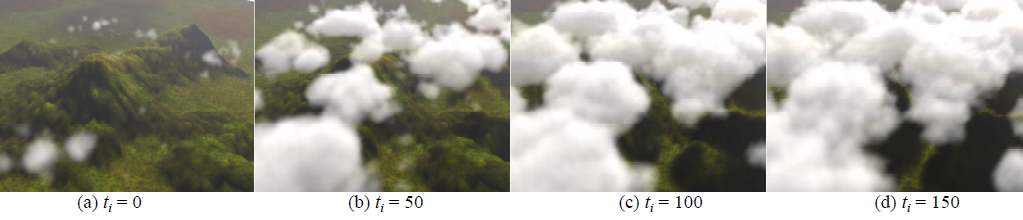
\includegraphics[width=\textwidth]{images/Simple_Realistic_Animation_of_Clouds.PNG}
  \caption{\citet{DobashiEtAl00}}
  \label{fig:Simple Realistic Animation of Clouds}
\end{figure}

The other method for testing the application is to test how much resources are being used by the application.
\citet*{MHarris01}, and \citet{Elek12} both used this method when evaluating their models.
This form of evaluation tests how efficient the application is when running in real time as well as concerns like the size of grid that can be used.
This can be accomplished using Nsight Visual Studio Edition (\citeyear{nvidiasight2013}) for debugging CUDA and profiling the application.